\documentclass[mathserif,serif,10pt]{beamer}
\usepackage[T2A,T1]{fontenc}
\usepackage[utf8]{inputenc}
\usepackage[ukrainian]{babel}
\usepackage{pgfplots}
\usepackage{hyperref}
%\usepackage[margin=0.6in]{geometry}

\begin{document}

\begin{frame}
 \frametitle{Метод 1}
Нуклеотидам A, G, C і T ставляться у відповідність вектори: A $(1,0.8)$, G $(1,0.6)$, C $(1,0.4)$, T $(1,0.2)$.
Послідовність отримуємо, сумуючи вектори, що відповідають нуклеотидам з послідовності.
\begin{figure}
\begin{center}
\begin{tikzpicture}
\begin{axis}[xmin=0,ymin=0]
\addplot[color=red,mark=x] coordinates {
(0,0)
(1.0, 0.8)
(2.0, 1.0)
(3.0, 1.6)
(4.0, 2.0)
(5.0, 2.2)
(6.0, 2.8)
(7.0, 3.2)
(8.0, 3.4)
(9.0, 4.0)
(10.0, 4.8)
};
\pgfplotsset{
after end axis/.code={
\node[black,above] at (axis cs:1,0.8){\small{$A$}};
\node[black,above] at (axis cs:2.0, 1.0){\small{$T$}};
\node[black,above] at (axis cs:3.0, 1.6){\small{$G$}};
\node[black,above] at (axis cs:4.0, 2.0){\small{$C$}};
\node[black,above] at (axis cs:5.0, 2.2){\small{$T$}};
\node[black,above] at (axis cs:6.0, 2.8){\small{$G$}};
\node[black,above] at (axis cs:7.0, 3.2){\small{$C$}};
\node[black,above] at (axis cs:8.0, 3.4){\small{$T$}};
\node[black,above] at (axis cs:9.0, 4.0){\small{$G$}};
\node[black,above] at (axis cs:10.0, 4.8){\small{$A$}};
}
}
\end{axis}
\end{tikzpicture}
\end{center}
\caption{Графічне представлення послідовності ATGCTGCTGA}
\label{fig:1}
\end{figure}
\end{frame}

\begin{frame}
\frametitle{Метод 2}
Спочатку використаємо попередній метод щоб отримати числову послідовність $(x_i,y_i)$. Далі використаємо наступну формулу для обчислення результуючої послідовності:
\[{x_i-\overrightarrow{y_i} \over{{1\over2}n(n+1)-y_n}},\]
де $\overrightarrow{y_i}$ це $y$-компонента вектора, що відповідає $i$-тому нуклеотиду при використанні методу 1, $n$ це розмір ДНК послідовності.
\end{frame}

\begin{frame}
\frametitle{Метод 3}
Нуклеотидам A, G, C, T ставимо у відповідність вектори $(-1,0)$, $(1,0)$,
$(0,1)$, $(0,-1)$. Починаємо з точки $(0,0)$ і рухаємось по відповіднім
векторам. Точки через які ми проходимо утворюють послідовність, причому точка
стільки разів зустрічається у послідовності, скільки разів ми в неї потрапили.
\begin{figure}[h!]
\centering
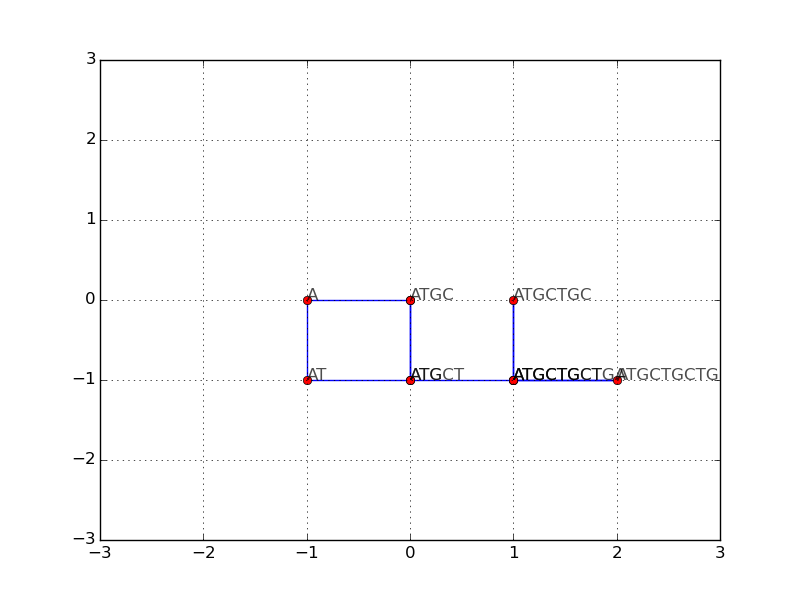
\includegraphics[width=0.65\textwidth]{meth3}
\caption{Графічне представлення послідовності ATGCTGCTGA}
\end{figure}
\end{frame}

\begin{frame}
\frametitle{Метод 4}
Розташовуємо нуклеотиди у вершинах квадрата зі стороною 1: A=$(0,0)$,
G=$(1,1)$, C=$(0,1)$, T=$(1,0)$. Координати послідовності рахуються ітеративно,
рухаючись на половину відстані між попередньою позицією і точкою квадрата, якій
відповідає наступний нуклеотид у напрямку цієї точки. Ітеративну процедуру
можна задати наступним чином:
\[p_i = p_{i-1}-0.5(p_{i-1}-g_i)\]
\[i=1,...,n; p_0=(0.5,0.5),\]
де $g_i$ - координати, що відповідають $i$-тому нуклеотиду, $n$ - довжина послідовності ДНК.
\end{frame}

\begin{frame}
\frametitle{Метод 4}
\begin{figure}[h!]
\begin{center}
\begin{tikzpicture}
\begin{axis}[xmin=0,xmax=1,ymin=0,ymax=1]
\addplot[color=red,mark=x] coordinates {
(0.5,0.5)
(0.25, 0.25)
(0.625, 0.125)
(0.8125, 0.5625)
(0.40625, 0.78125)
(0.703125, 0.390625)
(0.8515625, 0.6953125)
(0.42578125, 0.84765625)
(0.712890625, 0.423828125)
(0.8564453125, 0.7119140625)
(0.42822265625, 0.35595703125)
};
\pgfplotsset{
after end axis/.code={
\node[black,above] at (axis cs:0.25, 0.25){\small{$A$}};
\node[black,above] at (axis cs:0.62, 0.12){\small{$T$}};
\node[black,right] at (axis cs:0.81, 0.56){\small{$G$}};
\node[black,above] at (axis cs:0.40, 0.78){\small{$C$}};
\node[black,left] at (axis cs:0.70, 0.39){\small{$T$}};
\node[black,above] at (axis cs:0.85, 0.69){\small{$G$}};
\node[black,above] at (axis cs:0.42, 0.84){\small{$C$}};
\node[black,below] at (axis cs:0.71, 0.42){\small{$T$}};
\node[black,right] at (axis cs:0.85, 0.71){\small{$G$}};
\node[black,above] at (axis cs:0.42, 0.35){\small{$A$}};
}
}
\end{axis}
\end{tikzpicture}
\end{center}
\caption{Графічне представлення послідовності ATGCTGCTGA}
\label{fig:f2}
\end{figure}
\end{frame}

\begin{frame}
\frametitle{Метод 5,6}

Використовуємо попередній метод, щоб отримати послідовність $p_i$, отримуємо результуючу, як суму всіх попередніх:
\[z_i = \sum_{j=1}^{i} p_i\]

Отримуємо за допомогою методу 4 послідовність $p_i$ і, щоб отримати результуючу послідовність, кожній точці ставимо у відповідність число:
\[z_i = x_i + y_i,\]
де $p_i = (x_i,y_i)$.
\end{frame}

\begin{frame}
\frametitle{Метод 7}
Нуклеотидам A,C ставимо у відповідність $-1$, а нуклеотидам T,G ставимо у відповідність $1$. Починаючи з точки $0$ рухаємось ітеративно:
\[p_i = p_{i-1} - {(g_i-p_{i-1}) \over{2}}sign(g_i)\]
де $g_i$ число яке відвідає $i$-тому нуклеотиду. Тобто ми, подібно до методу 4, рухаємося на пів відстань до числа яке відповідає $i$-тому нуклеотиду.

\begin{figure}[h!]
\centering
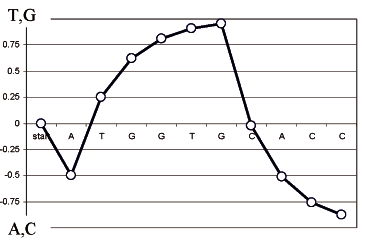
\includegraphics[width=0.55\textwidth]{meth7}
\caption{Графічне представлення послідовності ATGGTGCACC}
\end{figure}

\end{frame}

\begin{frame}
\frametitle{$p$-статистика}
$G$ і $G'$-генеральні сукупності.
$x=(x_1,...,x_n)\in G$ і $x'=(x_1',...,x_m')\in G'$, $x_{(1)}<...<x_{(n)}$, $x_{(1)}'<...<x_{(n)}'$ - порядкові статистики.
Припустимо, що $F_G(u) = F_{G'}(u)$.
$A_{ij}^{(k)} = \left\{x_k' \in \left(x_{(i)}, x_{(j)}\right)\right\}$.
Якщо $F_G(u) = F_{G'}(u)$:
\[P\left(A_{ij}^{(k)}\right) = P\left(x_k' \in \left(x_{(i)}, x_{(j)}\right)\right) = p_{ij}^{(n)} = {{j-i}\over{n+1}} = {{q}\over{n+1}}, q = j-i\]
\begin{equation}\label{eq:p1}
p_{ij}^{(1)} = {{h_{ij}^{(n)}m+g^2/2-g\sqrt{h_{ij}^{(n)}(1-h)m+g^2/4}}\over{m+g^2}},
\end{equation}
\begin{equation}\label{eq:p2}
p_{ij}^{(2)} = {{h_{ij}^{(n)}m+g^2/2+g\sqrt{h_{ij}^{(n)}(1-h)m+g^2/4}}\over{m+g^2}},
\end{equation}
де $h_{ij}^{(n)}$ — частота події $A_{ij}^{(n)}$
в $m$ випробуваннях.
$N$ кількість інтервалів
$I_{ij}^{(n,m)} = \left(p_{ij}^{(1)},p_{ij}^{(2)}\right)$ ($N=n(n-1)/2$) і $L$ -
кількість інтервалів $I_{ij}^{(n,m)}$, які містять ймовірності $p_{ij}^{(n)}$.
$h^{(n,m)}= \rho(x,x') = {L\over{N}}$ будемо називати $p$-статистикою.
\end{frame}

\begin{frame}
\frametitle{Модифікована $p$-статистика}
Нехай $t(x_k)$ - кратість вибіркового значення $x_k$
\[
p_{ij}=p\left(A_{ij}\right)=p\left(x^{*} \in (x_{(i)}, x_{(j)})\right) \approx
\gamma_i + \gamma_{i+1} + ... + \gamma_{j-1} + {{j-i}\over{n+1}},
\]
\[\gamma_{l} = \gamma \left(x_{(l)}\right) = {{t(x_{(l)})-1}\over{n+1}},\]
\end{frame}

\begin{frame}
\frametitle{Еліпси Петуніна}
\begin{figure}[h!]
\centering
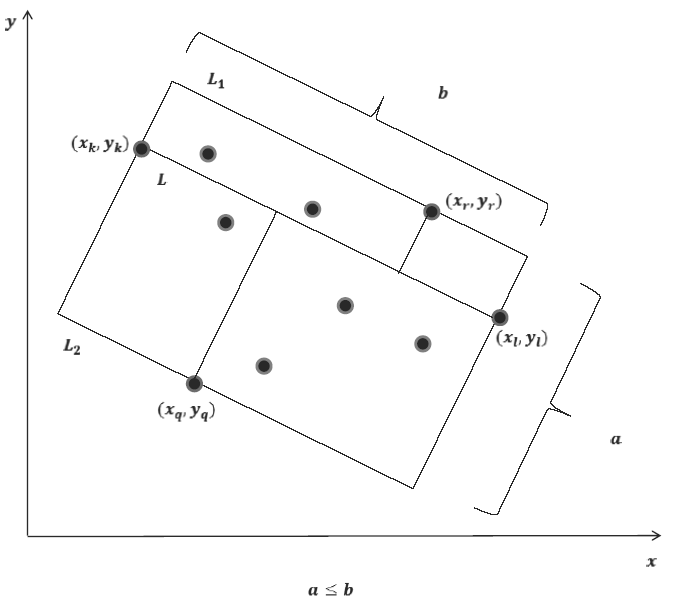
\includegraphics[width=0.55\textwidth]{pet1}
\end{figure}
\end{frame}

\begin{frame}
\frametitle{Еліпси Петуніна}
\begin{figure}[h!]
\centering
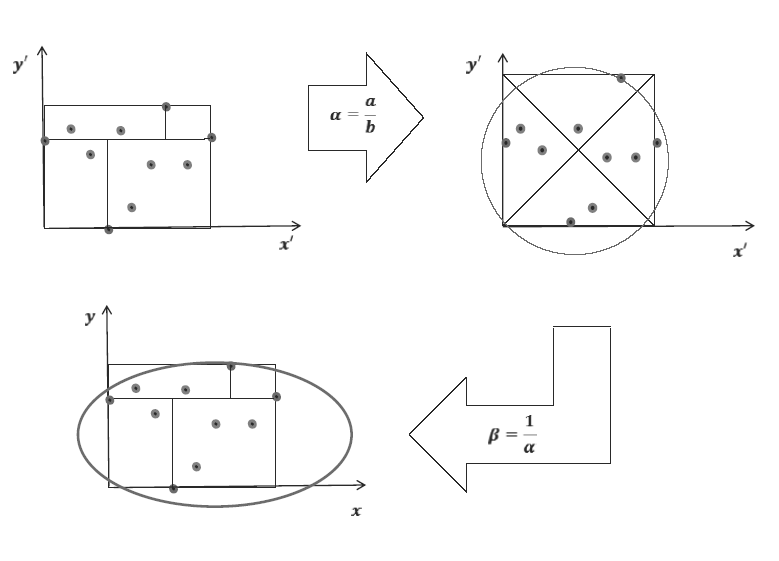
\includegraphics[width=1.0\textwidth]{pet2}
\end{figure}
\end{frame}

\begin{frame}
\frametitle{Еліпси Петуніна}
\begin{figure}[h!]
\centering
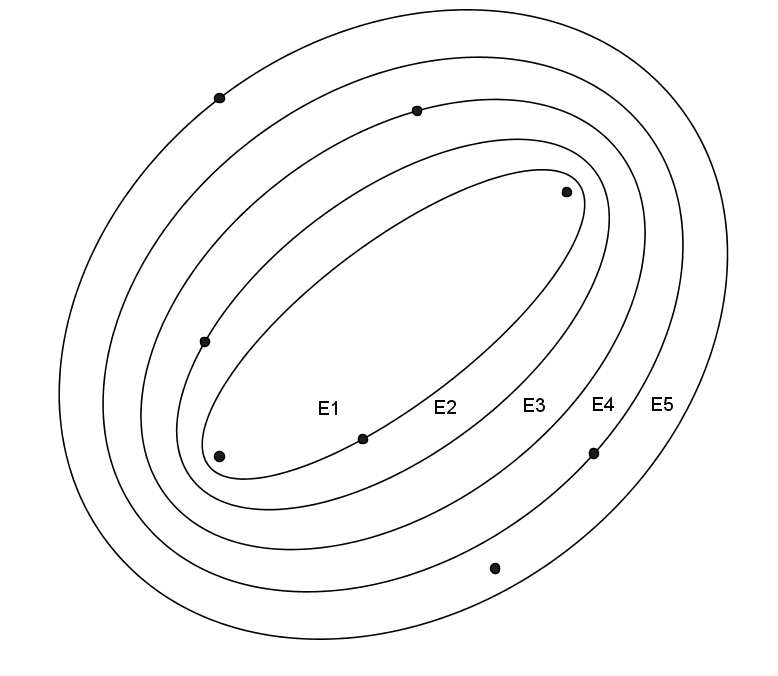
\includegraphics[width=0.8\textwidth]{pet3}
\end{figure}
\end{frame}

\begin{frame}
\frametitle{Еліпси Петуніна}
При побудові $p$-статистики варіаційному ряду вибірок
$\overrightarrow{x}_{(1)} \preceq \overrightarrow{x}_{(2)} \preceq
... \preceq \overrightarrow{x}_{(n)}$ поставимо у відповідність послідовність
вкладених еліпсоїдів $E_{(1)} \subset E_{(2)} \subset ... \subset E_{(n)}$. Ймовірність того, що елемент $\overrightarrow{x}$ із генеральної сукупності $G$ задовольняє умові $\overrightarrow{x}_{(i)} \preceq \overrightarrow{x} \preceq
\overrightarrow{x}_{(j)}$, рівна ймовірності потрапити між еліпсами $E_{(i)}$ і $E_{(j)}$, тобто $j-i \over n+1$. Ця умова дозволяє побудувати $p$-статистику для багатовимірного випадку. \par
Таким чином будуємо $p$-статистику як завжди, тільки подія $A_{ij}^{(k)}$ буде полягати в тому, що $x_k'$ попаде в область $E_{(j)} \setminus E_{(i)}$.
\end{frame}

\begin{frame}
\frametitle{Результати}
\begin{table}[h!]
\begin{center}
\begin{tabular}{|c|c|c|c|c|c|c|}
\hline
- & gallus & rat & rabbit & human & duck & gorilla \\ \hline
gallus & - & 0.009 & 0.009 & 0.0045 & 0.01365 & 0.01811 \\ \hline
rat & - & - & 0.00869 & 0.00633 & 0.00797 & 0.0088 \\ \hline
rabbit & - & - & - & 0.00619 & 0.00996 & 0.011 \\ \hline
human & - & - & - & - & 0.00595 & 0.00441 \\ \hline
duck & - & - & - & - & - & 0.01754 \\ \hline
gorilla & - & - & - & - & - & - \\ \hline
\end{tabular}
\end{center}
\caption{$p$-статистики при представленні ДНК методом 1}
\label{table:res1}
\end{table}

\begin{table}[h!]
\begin{center}
\begin{tabular}{|c|c|c|c|c|c|c|}
\hline
- & gallus & rat & rabbit & human & duck & gorilla \\ \hline
gallus & - & 0.03221 & 0.03896 & 0.0177 & 0.07635 & 0.09232 \\ \hline
rat & - & - & 0.30299 & 0.07789 & 0.06678 & 0.05958 \\ \hline
rabbit & - & - & - & 0.05915 & 0.09386 & 0.08013 \\ \hline
human & - & - & - & - & 0.03564 & 0.03172 \\ \hline
duck & - & - & - & - & - & 0.72326 \\ \hline
gorilla & - & - & - & - & - & - \\ \hline
\end{tabular}
\end{center}
\caption{$p$-статистики при представленні ДНК методом 2}
\label{table:res2}
\end{table}

\end{frame}
\begin{frame}
\frametitle{Результати}

\begin{table}[h!]
\begin{center}
\begin{tabular}{|c|c|c|c|c|c|c|}
\hline
- & gallus & rat & rabbit & human & duck & gorilla \\ \hline
gallus & - & 0.01839 & 0.01839 & 0.00922 & 0.02752 & 0.04045 \\ \hline
rat & - & - & 0.03393 & 0.01004 & 0.02045 & 0.0182 \\ \hline
rabbit & - & - & - & 0.0105 & 0.02045 & 0.0182 \\ \hline
human & - & - & - & - & 0.00821 & 0.00912 \\ \hline
duck & - & - & - & - & - & 0.03174 \\ \hline
gorilla & - & - & - & - & - & - \\ \hline
\end{tabular}
\end{center}
\caption{$p$-статистики при представленні ДНК методом 3}
\label{table:res3}
\end{table}

\begin{table}[h!]
\begin{center}
\begin{tabular}{|c|c|c|c|c|c|c|}
\hline
- & gallus & rat & rabbit & human & duck & gorilla \\ \hline
gallus & - & 0.20654 & 0.20122 & 0.18473 & 0.28257 & 0.32461 \\ \hline
rat & - & - & 0.15438 & 0.12881 & 0.22096 & 0.20542 \\ \hline
rabbit & - & - & - & 0.1298 & 0.2198 & 0.21226 \\ \hline
human & - & - & - & - & 0.16495 & 0.16271 \\ \hline
duck & - & - & - & - & - & 0.22192 \\ \hline
gorilla & - & - & - & - & - & - \\ \hline
\end{tabular}
\end{center}
\caption{$p$-статистики при представленні ДНК методом 4}
\label{table:res4}
\end{table}

\end{frame}
\begin{frame}
\frametitle{Результати}


\begin{table}[h!]
\begin{center}
\begin{tabular}{|c|c|c|c|c|c|c|}
\hline
- & gallus & rat & rabbit & human & duck & gorilla \\ \hline
gallus & - & 0.009 & 0.00902 & 0.0045 & 0.01367 & 0.01821 \\ \hline
rat & - & - & 0.00877 & 0.00635 & 0.00801 & 0.00882 \\ \hline
rabbit & - & - & - & 0.0062 & 0.01 & 0.01101 \\ \hline
human & - & - & - & - & 0.00595 & 0.00446 \\ \hline
duck & - & - & - & - & - & 0.01759 \\ \hline
gorilla & - & - & - & - & - & - \\ \hline
\end{tabular}
\end{center}
\caption{$p$-статистики при представленні ДНК методом 5}
\label{table:res5}
\end{table}

\begin{table}[h!]
\begin{center}
\begin{tabular}{|c|c|c|c|c|c|c|}
\hline
- & gallus & rat & rabbit & human & duck & gorilla \\ \hline
gallus & - & 0.41829 & 0.46788 & 0.18442 & 0.35209 & 0.46493 \\ \hline
rat & - & - & 0.995 & 0.34451 & 0.50635 & 0.43534 \\ \hline
rabbit & - & - & - & 0.37162 & 0.52875 & 0.60944 \\ \hline
human & - & - & - & - & 0.8112 & 0.38868 \\ \hline
duck & - & - & - & - & - & 0.49541 \\ \hline
gorilla & - & - & - & - & - & - \\ \hline
\end{tabular}
\end{center}
\caption{$p$-статистики при представленні ДНК методом 6}
\label{table:res6}
\end{table}

\end{frame}
\begin{frame}
\frametitle{Результати}

\begin{table}[h!]
\begin{center}
\begin{tabular}{|c|c|c|c|c|c|c|}
\hline
- & gallus & rat & rabbit & human & duck & gorilla \\ \hline
gallus & - & 0.59803 & 0.56986 & 0.90713 & 0.88857 & 0.94818 \\ \hline
rat & - & - & 0.99778 & 0.56047 & 0.39723 & 0.40133 \\ \hline
rabbit & - & - & - & 0.42243 & 0.38003 & 0.3786 \\ \hline
human & - & - & - & - & 0.59813 & 0.77453 \\ \hline
duck & - & - & - & - & - & 0.95202 \\ \hline
gorilla & - & - & - & - & - & - \\ \hline
\end{tabular}
\end{center}
\caption{$p$-статистики при представленні ДНК методом 7}
\label{table:res7}
\end{table}
\end{frame}

\begin{frame}
\frametitle{Висновки}
Алгоритм побудови $p$-статистик для послідовностей ДНК досить повільний. Тому не доцільно його застосовувати при послідовностях, довжина яких перевищує $10^3$.
\par

Результати суперечать інтуїтивному уявленню, про зв’язок близькості геномних послідовностей і міжвидової близькості.
\end{frame}

\begin{thebibliography}{9}

\begin{frame}
\frametitle{Література}

\bibitem{l1}
Chenglong Yu, Mo Deng, Stephen S.-T. Yau,
DNA sequence comparison by a novel probabilistic method,
Information Sciences 181 (2011) 1484–1492
\bibitem{l2}
Dorota Bielinska-Waz, Timothy Clark, Piotr Waz, Wiesław Nowak, Ashesh Nandy,
2D-dynamic representation of DNA sequences,
Chemical Physics Letters 442 (2007) 140–144
\bibitem{l3}
Wei Deng and Yihui Luan,
Hindawi Publishing Corporation,
Analysis of Similarity/Dissimilarity of DNA Sequences Based on Chaos Game Representation,
Abstract and Applied Analysis,
Volume 2013, Article ID 926519, 6 pages,
http://dx.doi.org/10.1155/2013/926519
\end{frame}
\begin{frame}
\frametitle{Література}
\bibitem{l4}
Jure Zupan and Milan Randic,
Algorithm for Coding DNA Sequences into “Spectrum-like” and “Zigzag” Representations,
J. Chem. Inf. Model. 2005, 45, 309-313
\bibitem{l5}
Д. А. Клюшин, Ю. И. Петунин,
Непараметрический Критерий Эквивалентности Генеральных Совокупностей, основанный На Мере Близости Между Выборками,
ДК 519.21
\bibitem{l6}
Д. А. Клюшин, М. В. Присяжная,
Многомерное ранжирование с помощью эллипсов Петунина,
Журнал обчисл. та прикл. матем. № 4(114) 2013, стор. 1-7,
УДК 519.71
\bibitem{l7}
Дмитро А. Клюшин,
Міра близькості між виборками, що містять атоми,
Вісник Київського університету,
Серія: фізико-математичні науки,
2005, 3,
УДК 519.9

\end{frame}
\end{thebibliography}



\end{document}
